\documentclass[11pt]{article}
\usepackage{amsmath}
\usepackage{graphicx}
\usepackage{longtable}
\usepackage[left=3cm, right=3cm]{geometry}
\usepackage{titling}

\setlength{\droptitle}{-5em}

\begin{document}

\title{\LARGE{\textbf{Query Optimisation Lab Report}}\vspace{-2em}}
\date{}
\maketitle



\setlength{\parindent}{0pt}
\section{Query Analysis}

The queries will be run on the Mondial10 database. The \texttt{real} time will be used to measure query execution times, as it represents
the total time from the user's perspective. It includes external delays, which can occur when queries require disk access, such delays
are not captured in \texttt{user} or \texttt{sys} times.
\\ \\ 
All of the measurements are taken on an Acer Aspire A515-44, 2.38 GHz AMD Ryzen 5 with 8 GB RAM with 512 GB Flash Storage running Windows 11
V10.0.22631 and SQLite version 3.47.0.


\subsection{Query Pair 1: Auto Index Optimisation}

SQLite is able to optimise queries using automatic indices, which can significantly improve performance by avoiding full
table scans during lookups or joins. In this query pair, one will be optimisable where SQLite can create an index,
while the other will not be optimisable due to the use of transformations on indexed columns.
\\ \\
The queries will select cities with a population greater than 1,000,000, along with the country that the city belongs to.

\subsubsection{Query 1A: Optimisable by using automatic index}

\begin{verbatim}
SELECT c.Name, ci.Name
FROM Country c
JOIN City ci ON ci.Country = c.Code
WHERE ci.Population > 1000000;
\end{verbatim}

\noindent This query would be optimisable by SQLite, as the optimiser would create an auto index on the country table when joining the city table.

\subsubsection{Query 1B: Transformation on JOIN Column - Not Optimisable}

\begin{verbatim}
SELECT c.Name, ci.Name
FROM Country c
JOIN City ci ON CAST(ci.Country AS TEXT) = CAST(c.Code AS TEXT)
WHERE ci.Population > 1000000;
\end{verbatim}

\noindent This query is similar to 1A, except that both columns in the \texttt{JOIN} are type-cast to \texttt{TEXT}. 

\subsubsection{Hypothesis}

SQLite should optimise 1A by creating an automatic index on the \texttt{Country.Code} column for the \texttt{JOIN} and possibly
on \texttt{City.Population} for filtering. This should result in an efficient query plan.
\\ \\
Because of the use of \texttt{CAST} in the \texttt{JOIN} condition in 1B, SQLite should not be able to create any indices on
\texttt{Country.Code} or \texttt{City.Country}. Indices only work on raw column values, and so this query should not be optimisable since the
\texttt{CAST} function transforms the two columns. Instead, it should perform full table scans on both tables, leading to a less efficient
query plan with higher execution times.

\subsubsection{Results and Discussion}

\begin{longtable}{|l|l|l|l|l|l|l|}
\hline
Query & Run 1 (s) & Run 2 (s) & Run 3 (s) & Run 4 (s) & Run 5 (s) & Average (s) \\
\hline
\endfirsthead
\hline
Query & Run 1 (s) & Run 2 (s) & Run 3 (s) & Run 4 (s) & Run 5 (s) & Average (s) \\
\hline
\endhead
Query 1A & 0.067 & 0.067 & 0.065 & 0.066 & 0.065 & 0.0660 \\
Query 1B & 0.806 & 0.805 & 0.800 & 0.814 & 0.808 & 0.8066 \\
\hline
\caption{Execution Times on Mondial10 Database}
\end{longtable}


\textbf{Query Execution Plan of 1A:}
\begin{verbatim}
|--SCAN ci
`--SEARCH c USING AUTOMATIC COVERING INDEX (Code=?)
\end{verbatim}

\textbf{Query Execution Plan of 1B:}
\begin{verbatim}
|--SCAN ci
`--SCAN c
\end{verbatim}

\noindent Table 1 shows that 1A's average execution time (0.0660) was around 91.8\% faster than 1B (0.8066). 1A benefited from SQLite's use of automatic
covering indices, with an index on \texttt{Country.Code} to allow searching, this plan would have been chosen based on factors such as the cost of scanning, table sizes
and selectivity.
\\ \\
In contrast, 1B relied on full table scans due to type-cast transformations on the \texttt{JOIN} columns, preventing index usage. Indices are more efficient
as they reduce the search space, allowing SQLite to directly locate relevant rows and minimise comparisons and disk I/O. Full table scans (as shown in 1B's execution plan), however,
process all rows sequentially, which is costly in a large database. The \texttt{CAST} operation forces SQLite to treat the columns as derived expressions, making them ineligible for indexing.

\subsection{Query Pair 2: Subquery Optimisation}

This query pair explores how SQLite optimises nested subqueries, comparing a derived table approach and a correlated subquery.
Both queries aim to retrieve the names of countries alongside the average population of their cities, but their performance depends significantly
on how SQLite's optimiser processes them.

\subsubsection{Query 2A: Optimisable by Query Flattening or Co-Routines}

\begin{verbatim}
SELECT c.Name, s.AvgPop AS AverageCityPopulation
FROM Country c, (
    SELECT ci.Country, AVG(ci.Population) AS AvgPop
    FROM City ci
    GROUP BY ci.Country
) s
WHERE c.Code = s.Country;
\end{verbatim}

\noindent This query calculates the average population of cities by grouping the \texttt{City} table in a subquery within the \texttt{FROM} clause.
The result is treated as a derived table (\texttt{s}) and joined with the \texttt{Country} table. 

\subsubsection{Query 2B: Correlated Subquery - Not Optimisable}

\begin{verbatim}
SELECT c.Name, 
       (SELECT AVG(Population) 
        FROM City 
        WHERE City.Country = c.Code) AS AverageCityPopulation
FROM Country c;
\end{verbatim}

\noindent Query 2B uses a correlated subquery within the \texttt{SELECT} clause. For every row in the \texttt{Country} table, the subquery calculates
the average city population by scanning the City table. 

\subsubsection{Hypothesis}

The SQLite optimiser can optimise 2A through query flattening or co-routine execution. Query flattening transforms the subquery into a
\texttt{JOIN}, eliminating the need for separate execution and enabling more efficient data retrieval. Alternatively, SQLite may use co-routines, which
process the subquery in parallel with the outer query, delivering rows incrementally as needed. Both techniques should enhance performance.
\\ \\
In contrast, 2B's correlated subquery structure should hinder optimisation. The subquery must be evaluated separately for each row of the
\texttt{Country} table, as it references values from the outer query. This dependency should lead to multiple scans of the \texttt{City} table,
increasing execution time in comparison to 2A.

\subsubsection{Results and Discussion}

\begin{longtable}{|l|l|l|l|l|l|l|}
\hline
Query & Run 1 (s) & Run 2 (s) & Run 3 (s) & Run 4 (s) & Run 5 (s) & Average (s) \\
\hline
\endfirsthead
\hline
Query & Run 1 (s) & Run 2 (s) & Run 3 (s) & Run 4 (s) & Run 5 (s) & Average (s) \\
\hline
\endhead
Query 2A & 0.059 & 0.061 & 0.059 & 0.061 & 0.059 & 0.0598 \\
Query 2B & 5.266 & 5.245 & 5.248 & 5.306 & 5.353 & 5.2836 \\
\hline
\caption{Execution Times on Mondial10 Database}
\end{longtable}


\textbf{Query Execution Plan of 2A:}
\begin{verbatim}
|--CO-ROUTINE s
|  |--SCAN ci
|  `--USE TEMP B-TREE FOR GROUP BY
|--SCAN c
`--SEARCH s USING AUTOMATIC COVERING INDEX (Country=?)
\end{verbatim}


\textbf{Query Execution Plan of 2B:}
\begin{verbatim}
|--SCAN c
`--CORRELATED SCALAR SUBQUERY 1
    `--SCAN City
\end{verbatim}

\noindent From the results in Table 2, we can observe that query 2A performed significantly better than 2B. There was approximately a 98\%
decrease in execution time from query 2B to 2A.
\\ \\
The query plans show that the SQLite optimiser was able to effectively utilise co-routines in 2A to run the subquery once in parallel with the outer query.
This allows the outer query to process rows as they are needed without waiting for the entire subquery to complete. The optimiser also uses a temporary B-Tree
to optimise aggregation (\texttt{GROUP BY}), and uses an automatic covering index to optimise joins between the subquery and the outer query.
\\ \\
In the execution plan of 2B, the optimiser is not able to use parallelism or indexing. The correlated subquery in the \texttt{SELECT} clause makes
the subquery dependent on the current row of the \texttt{Country} table, forcing it to scan the entire \texttt{City} table for each row in \texttt{Country}. This explains the
increased execution time observed.


\subsection{Query Pair 3: JOIN Order Optimisation}

This query pair examines SQLite's join reordering optimisation, using different join strategies to retrieve countries with populations over 10,000,000,
their capitals, and continents they belong to, with continent area being over 30,000,000 km².

\subsubsection{Query 3A: JOIN - Optimisable by Reordering}

\begin{verbatim}
SELECT Country.Name, City.Name, City.Population, Continent.Name
FROM Country
JOIN encompasses ON encompasses.Country = Country.Code
JOIN Continent ON encompasses.Continent = Continent.Name
JOIN City ON City.Name = Country.Capital AND City.country = Country.Code
WHERE Continent.Area > 30000000 AND Country.Population > 10000000;
\end{verbatim}

\noindent This query involves \texttt{(INNER) JOIN}s between the \texttt{Country, encompasses, Continent,} and \texttt{City} tables.

\subsubsection{Query 3B: CROSS JOIN - Order Not Optimisable}

\begin{verbatim}
SELECT Country.Name, City.Name, City.Population, Continent.Name
FROM City
CROSS JOIN encompasses
CROSS JOIN Continent
CROSS JOIN Country
WHERE Continent.Area > 30000000 AND Country.Population > 10000000
    AND encompasses.Country = Country.Code
    AND encompasses.Continent = Continent.Name
    AND City.Name = Country.Capital
    AND City.country = Country.Code;
\end{verbatim}

\noindent In this query, \texttt{CROSS JOIN}s are used between the \texttt{City, encompasses, Continent,} and \texttt{Country} tables. The filtering conditions in the
\texttt{WHERE} clause are applied to ensure that valid rows are returned, and matches results from 3A.

\subsubsection{Hypothesis}

SQLite should optimise 3A by selecting an efficient join order through join reordering. Since \texttt{(INNER) JOIN}s are commutative, the
optimiser can reorder the joins to find the most efficient execution order. The query planner should evaluate the cost of
potential join orders, considering statistics and factors such as the table sizes, available indices, and filtering conditions, and choose an optimal join order.
\\ \\
On the other hand, 3B uses \texttt{CROSS JOIN}s, which do not allow join reordering. This means that the tables must be processed in the order they appear,
the optimiser would not be able to adjust the order to minimise work. This approach should lead to larger intermediate results and require
more processing time, resulting in a less efficient query plan compared to 3A.

\subsubsection{Results and Discussion}

\begin{longtable}{|l|l|l|l|l|l|l|}
\hline
Query & Run 1 (s) & Run 2 (s) & Run 3 (s) & Run 4 (s) & Run 5 (s) & Average (s) \\
\hline
\endfirsthead
\hline
Query & Run 1 (s) & Run 2 (s) & Run 3 (s) & Run 4 (s) & Run 5 (s) & Average (s) \\
\hline
\endhead
Query 3A & 1.180 & 1.162 & 1.195 & 1.178 & 1.184 & 1.1798 \\
Query 3B & 7.543 & 7.161 & 7.088 & 7.102 & 7.263 & 7.2314 \\
\hline
\caption{Execution Times on Mondial10 Database}
\end{longtable}


\textbf{Query Execution Plan of 3A:}
\begin{verbatim}
|--SCAN Country
|--SEARCH encompasses USING AUTOMATIC COVERING INDEX (Country=?)
|--SEARCH Continent USING AUTOMATIC PARTIAL COVERING INDEX (Name=?)
`--SEARCH City USING AUTOMATIC COVERING INDEX (Name=? AND Country=?)
\end{verbatim}


\textbf{Query Execution Plan of 3B:}
\begin{verbatim}
|--SCAN City
|--SCAN encompasses
|--SEARCH Continent USING AUTOMATIC PARTIAL COVERING INDEX (Name=?)
`--SEARCH Country USING AUTOMATIC PARTIAL COVERING INDEX (Code=? AND Capital=?)
\end{verbatim}

\noindent Query 3A's average execution time (1.1798) is around 83\% faster than 3B, which takes approximately 6.1 seconds longer.
3A benefits from join reordering, which allows SQLite to explore efficient join sequences based on table sizes, filtering conditions,
and available indexes. It is also able to scan one table and create indices for the subsequent joins. The indices allow searching, which will
only process relevant rows, instead of processing all rows in a scan. This results in significantly faster execution, as the intermediate data processed at each step is minimised.
\\ \\
Query 3B, on the other hand, suffers from the rigidity of \texttt{CROSS JOIN}s, which don't allow reordering. The query generates a Cartesian product
of all rows from the tables, leading to larger intermediate results. It does however use automatic indices for the filtering
in the \texttt{Country} and \texttt{Continent} table, this is probably influenced by optimising the filters in the \texttt{WHERE} clause, which are similar
to those that would appear in the \texttt{ON} clause of a \texttt{JOIN}.

\section{Reflection}

\begin{figure}
    \centering
    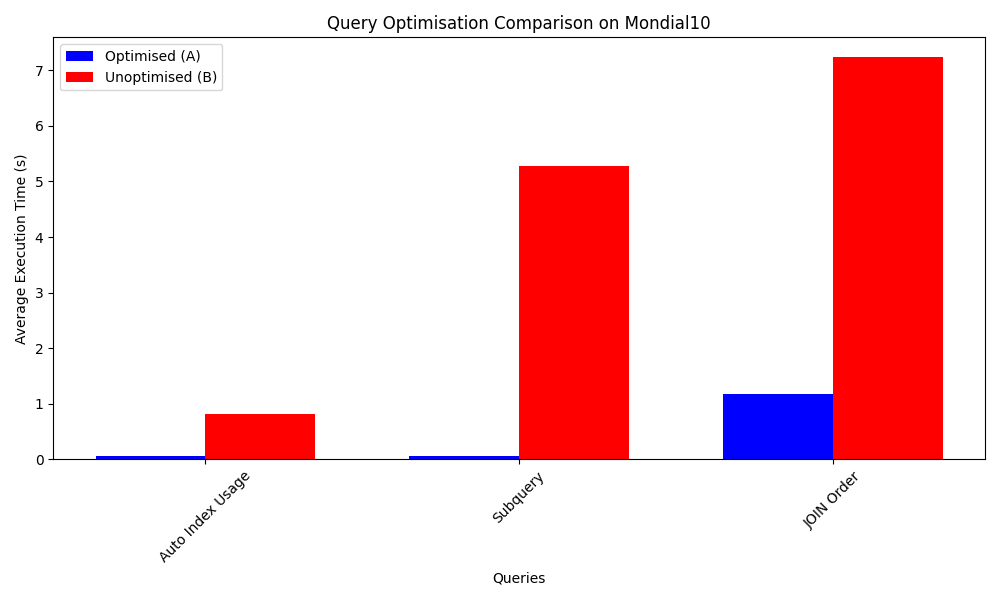
\includegraphics[width=0.9\linewidth]{query_execution_times.png}
    \caption{Query Pairs Execution Time Bar Plot}
    \label{fig:plot}
\end{figure}

Figure 1 illustrates the impact of SQLite's query optimisation techniques across the three scenarios. All of the optimised queries show a clear
reduction in time in comparison to their unoptimised counterparts. The index usage and subquery optimisation queries show near-instant execution with times less than 0.1 seconds. This is because they directly reduce
redundant operations, such as scanning the same table multiple times or evaluating intermediate results unnecessarily.
The difference in the join reordering queries is relatively modest compared to the other scenarios. The number of joins involved could explain
the greater execution times.
\\ \\
The experimentation also emphasises the need for developers to write queries that align with database optimisation strategies. Avoiding pitfalls like correlated subqueries ensures scalability,
particularly with a large database, as seen in query 2B. Similarly, leveraging \texttt{JOIN}s and understanding join reordering allows query planners to minimise intermediate results, improving performance,
as demonstrated in query 3A. Developers should also design queries to utilise indexing effectively, avoiding transformations on indexed columns, as highlighted in query 1B. By adopting these best practices,
developers can reduce execution times, optimise resource usage, and ensure their applications perform efficiently, even with complex queries and extensive data.
\\ \\
However, the experiment has limitations in fully accounting for optimisation performance, highlighting the need for tailored query design. All of the queries were run on the Mondial10 database, smaller
or larger databases could amplify or reveal shortcomings of these optimisations. For example, there might not be a huge difference between using and not using
an automatic index on a smaller database. Furthermore, the optimiser uses heuristics and statistics about the database to choose an optimisation
strategy, this may lead to varying optimisation strategies depending on database sizes. Uneven or skewed data distributions further complicate performance, sparse tables may weaken index efficiency,
while clustered or repetitive data might amplify indexing benefits but reduce join reordering effectiveness.

\end{document}